\chapter{Intégration}
\section{Introduction}

\paragraph{Motivation} : "Sommes continues" et Calcul d'aires.
\paragraph{Exemple} Soit un coureur.
Première course sur une machine.
\begin{itemize}
	\item $10km.h^{-1}$ pendant 20 minutes
	\item $12km.h^{-1}$ pendant 20 minutes
	\item $14km.h^{-1}$ pendant 20 minutes
\end{itemize}

Il aura donc parcouru : $(10*\frac{1}{3})+(12*\frac{1}{3})+(14*\frac{1}{3}) = 12 km$

2ème course

\begin{wrapfigure}[4]{r}{0pt}
	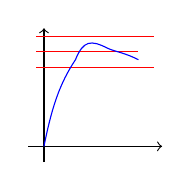
\begin{tikzpicture}
		\draw[->] (-0.2, 0) -- (1.5, 0);
		\draw[->] (0, -0.2) -- (0, 1.5);
		\draw[thin, red] (-0.1, 1) -- (1.4, 1);
		\draw[thin, red] (-0.1, 1.4) -- (1.4, 1.4);
		\draw[red] (-0.1, 1.2) -- (1.2, 1.2);

		\draw[blue] (0, 0) .. controls (0.1, 0.5) and (0.2, 0.8) .. (0.4, 1.1) .. controls (0.5, 1.35) and (0.6, 1.35) .. (0.8, 1.25) .. controls (0.9, 1.2) and (1, 1.2) .. (1.2, 1.1);

	\end{tikzpicture}
\end{wrapfigure}

La distance parcourue est la somme de la distance parcourue instantanément pour chaque instant.

"somme continue" : $\int_0^1 v(t)dt \rightarrow $ Calcul de l'air sous la courbe

\paragraph{2ème exemple}

\begin{wrapfigure}[5]{r}{0pt}
	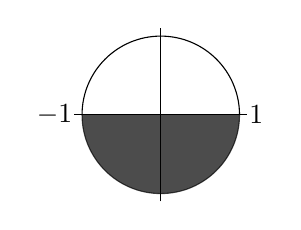
\begin{tikzpicture}
		\draw[] (-1.1, 0) -- (1.1, 0);
		\draw[] (0, -1.1) -- (0, 1.1);
		\draw[] (1, 0) arc (0:180:1);
		\draw[fill=black, opacity=0.7] (-1, 0) arc(180:360:1);
		\node[left] at (-1, 0) {$-1$};
		\node[right] at (1, 0) {$1$};
	\end{tikzpicture}
\end{wrapfigure}

On veut voir le cercle comme le graphe d'une fonction. On considère donc (par exemple) la partie supérieur du cercle.

L'équation du cercle centré en 0 et de rayon 1 est : \[\begin{array}{rcl}
		& x^2 + y^2 &= 1 \\
		\text{Ou encore } & y^2 &= 1 - x^2 \\
		\text{Ou encore } & y &= \pm\sqrt{1-x^2}\end{array}\]

On se restreint à $y \geq 0$ : $y = \sqrt{1-x^2}$
L'Aire(DemiCercle) = $\int_{-1}^{1} \sqrt{1-x^2} dx$

\subsection{Changement de variable}
\[\begin{array}{rcl}
		x &=& \cos t \\
		\cos:[1,\pi] & \rightarrow & [-1, 1]
\end{array}\]
Cette fonction est bijective et continue.
\[\begin{array}{rcl}
		dx &=& \frac{dx}{dt} \cdot dt \\
		   &=& (-\sin t)dt
\end{array}\]

\[\int_{-1}^1 \sqrt{1-x^2} dx = \int_\pi^0 \sqrt{1-\cos^2t} \cdot (-\sin t) dt\]

Or sur $[0, \pi], \sqrt{1-\cos^2 t} = \sqrt{\sin^2t} = |\sin t| = \sin t$
\[A = \int_\pi^0 -sin^2t dt = \int_0^\pi \sin^2t dt\]

\subsection{intégration par parties}
\paragraph{idée} $(f.g)' = f'g + fg'$ ~\\
donc : $fg' = (f.g)' - f'g$ ~\\
Avec la linéarité de l'intégrale ($\int (u+v)(t) dt = \int (u)(t) dt + \int (v)(t) dt$) ~\\
donc $\int_a^b fg'(t) dt = \int_a^b (fg)'(t)dt - \int_a^b f'g(t) dt$ ~\\
Ici, $A = \int_0^\pi \sin t \cdot \sin t dt$ ~\\

On pose $f'(t) = \sin t$ et g telle que $g'(t) = \sin (t)$ \[\int_0^\pi \sin t \sin t dt = \int_0^\pi[\sin t \cdot (-\cos t)] dt - \int_0^\pi[\cos t\cdot (-\cos t)dt]\] 

\[\begin{array}{rcl}
		\int_0^\pi \sin^2 t dt &=& \underbrace{[-\sin t \cos t]^\pi_0}{0} + \int_0^\pi \cos^2 t dt (1)
\end{array}\]

\subsection{} On sait que : $\forall t \in \mathbb{R}, \sin^2 t + \cos^2 t = 1$ ~\\

En particulier, \[\begin{array}{rcl}
		\int_0^\pi(\cos^2 t + \sin^2 t)dt &=& \int_0^\pi 1 dt \\
		\int_0^\pi \cos^2 t dt + \int_0^\pi \sin^2 t dt &=& \pi
\end{array}\]

\begin{wrapfigure}[3]{r}{0pt}
	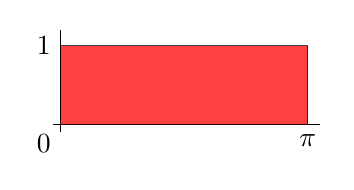
\begin{tikzpicture}
		\draw[] (-0.1, 0) -- (3.3, 0);
		\draw[] (0, -0.1) -- (0, 1.2);
		\node[below left] at (0, 0) {0};
		\node[below] at (3.14, 0) {$\pi$};
		\node[left] at (0, 1) {1};
		\draw[fill=red, opacity=0.75] (0, 0) rectangle (3.14, 1);
	\end{tikzpicture}
\end{wrapfigure}

\[\begin{array}{rcl}
		\int_0^\pi \cos^2 t dt + \int_0^\pi \sin^2 t dt &=& \pi \\
\text{D'après (1) } \int_0^\pi \cos^2 t dt &=& \int_0^\pi \sin^2t dt \end{array}\]
Donc \fbox{$2\int_0^\pi \sin^2 t dt = \pi \Rightarrow A = \int_0^\pi \sin^2 t dt = \frac{\pi}{2}$}

\section{Définition de l'intégrale}
\subsection{"Culture"}

\begin{wrapfigure}[6]{r}{0pt}
	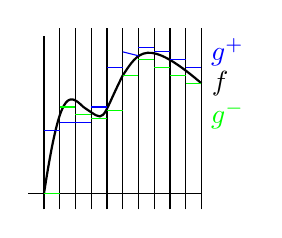
\begin{tikzpicture}
		\draw[] (-0.2, 0) -- (2, 0);
		\draw[] (0, -0.2) -- (0, 2);
		\foreach \x in {0.2, 0.4, ..., 2}{\draw[thin] (\x, -0.2) -- (\x, 2.1);}
		\draw[thick] (0, 0) .. controls (0.2, 1.3) and (0.3, 1.3) .. (0.5, 1.1) .. controls (0.8, 0.9) and (0.7, 0.9) .. (1, 1.5) .. controls (1.2, 1.8) and (1.3, 2) .. (2, 1.4) node [right]{$f$};

		\draw[green] (0,  0) -- (0.2, 0);
		\draw[green] (0.2,  1.1) -- (0.4, 1.1);
		\draw[green] (0.4,  1.0) -- (0.6, 1.0);
		\draw[green] (0.6,  0.95) -- (0.8, 0.95);
		\draw[green] (0.8,  1.05) -- (1, 1.05);
		\draw[green] (1,  1.5) -- (1.2, 1.5);
		\draw[green] (1.2,  1.7) -- (1.4, 1.7);
		\draw[green] (1.4,  1.6) -- (1.6, 1.6);
		\draw[green] (1.6,  1.5) -- (1.8, 1.5);
		\draw[green] (1.8,  1.4) -- (2, 1.4);
		\node[right, green] at (2, 1) {$g^-$};

		\draw[blue] (0,  0.8) -- (0.2, 0.8);
		\draw[blue] (0.2,  0.9) -- (0.4, 0.9);
		\draw[blue] (0.4,  0.9) -- (0.6, 0.9);
		\draw[blue] (0.6,  1.1) -- (0.8, 1.1);
		\draw[blue] (0.8,  1.6) -- (1, 1.6);
		\draw[blue] (1,  1.8) -- (1.2, 1.75);
		\draw[blue] (1.2,  1.85) -- (1.4, 1.85);
		\draw[blue] (1.4,  1.8) -- (1.6, 1.8);
		\draw[blue] (1.6,  1.7) -- (1.8, 1.7);
		\draw[blue] (1.8,  1.6) -- (2, 1.6);
		\node[right, blue] at (2, 1.8) {$g^+$};
	\end{tikzpicture}
\end{wrapfigure}

$\overbrace{\int_a^b g^- (t) dt}{\text{On sait calculer }} \leq \int_a^b f(t) dt \overbrace{\leq \int_a^b g^+ (t) dt}{\text{ Ça aussi }}$

\paragraph{Définition} $g: [a, b] \rightarrow \mathbb{R}$ est étapée s'il existe $a=t_0 < t_1<t_{n-1} < t_n = b$ ~\\
Si $\forall i \in [0, n-1], g_{|]t_i, t_{i+1}[}$

\paragraph{Définition 2} Si $g:[a, b] \rightarrow \mathbb{R}$ étapée, on définit : \[\int_a^b g(t)dt = \sum_{i=0}^{n-1} m_i \cdot (t_{i+1} - t_i)\]

\paragraph{Définition 3} Une fonction $f:[a, b] \rightarrow \mathbb{R}$ est \ul{integrable} s'il existe 2 suites de fonctions $(g^-_n)_{n \in \mathbb{N}},(g^+_n)_{n \in \mathbb{N}}$ étagées telles que : \[\left\{\begin{array}{c}
			-g^-_n \leq f \leq g^+_n \text{ et } \\
			\lim_{n \to +\infty} \int_a^b g^-_n(t) dt \text{ et } \lim_{n\to +\infty} \int_a^b g^+_n(t) dt
	\end{array}\right.\]
	existent et soient égales.

	Dans ce cas, on note cette limite commune $\lim_a^b f(t) dt$ ~\\ ~\\
	Par convention, si $a < b$, \[
	\int_b^a f(t)dt = -\int_a^b f(t) dt\]

	\paragraph{Théorème} Cette définition fonctionne, la démonstration est admise.

	\subsection{Retour à la vrai vie}

	\paragraph{Théorème} Si $f:[a, b] \rightarrow \mathbb{R}$ continue ou monotone, alors f est intégrable sur $[a, b]$
	\paragraph{Proposition} L'intégrale possède les propriétés suivantes.
	\begin{itemize}
		\item (positivité) si $f \geq 0$, alors $\int_a^b f(t)dt \geq 0$
		\item (Linéarité) $\left\{ \begin{array}{rcl}
					\int_a^b (f+g)(t) dt &=& \int_a^b f(t) dt + \int_a^b g(t) dt \\
				\int_a^b (\lambda f)(t) dt &=& \lambda (\int_a^b f(t)dt) \text{ avec } \lambda \in \mathbb{R}\end{array}\right.$
		\item $|\int_a^b f(t)dt| \leq \int_a^b |f(t)|dt$
	\end{itemize}

	\section{Liens entre primitives, intégrales (et dérivées)}

\paragraph{Définition} SOit $f:]a, b[ \rightarrow \mathbb{R}$, continue.
F est \ul{une primitive} de f si F dérivable sur $]a, b[$ et $F'=f$. 
\paragraph{Remarque} Alors F est $C^1(]a, b[)$

\paragraph{Théorème} \begin{enumerate}
\item Soit F et G des primitives de f sur $]a, b[$. Alors $F - G = constante$ sur $]a, b[$
\item Pour toute primitive de F de f sur $]a, b[, \int_a^b f(t)dt = F(b) - F(a)$
\end{enumerate}
